%& -shell-escape -enable-write18
\documentclass{standalone}
\usepackage{tikz}
\usetikzlibrary{external}
%\usepackage{caption}
\usetikzlibrary{shapes,arrows}

\newcommand{\mynodelabelfont}[1]{\fontsize{#1pt}{#1pt}\selectfont,yshift=-.2cm}

\begin{document}
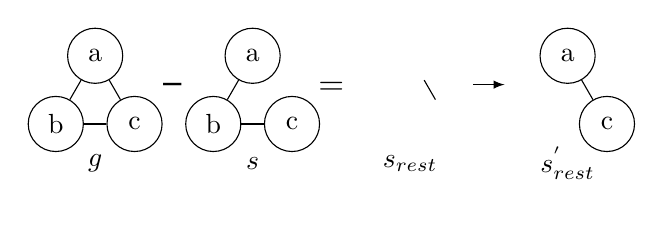
\begin{tikzpicture}[scale=1.0]
%[every node/.style={draw,circle}]
\tikzstyle{line} = [draw,-latex]
\tikzstyle{every node}=[draw,shape=circle,minimum size=0.7cm];
\colorlet{invisible}{white}
\colorlet{visible}{black}
%\tikzstyle{every label}=[text height=10pt];
\begin{scope}[xshift=0cm]
%\draw[help lines] (-1,-6) grid (10,6);
  \node (a) at (60:1cm) {a};
  \node (b) at (0:0cm)  {b};
  \node (c) at (0:1cm)  {c};
  	 \node [draw=none] (minus)  at   (1.5,.5){\scalebox{2.5}[1.5]{-} };
  	 \node [draw=none] (EdgeCutting) at (.5,-.5) {$g$};% edge cutting label

  \foreach \from/\to in {a/b,b/c,c/a}
    \draw (\from) -- (\to);
\end{scope}
\begin{scope}[xshift=2cm]
  \node (a) at (60:1cm) {a};
  \node (b) at (0:0cm)  {b};
   \node (c) at (0:1cm)  {c};
     \node [draw=none] (minus)  at   (1.5,.45){\scalebox{1.2}[1.2]{=} };
 	 \node [draw=none] (EdgeCutting) at (.5,-.5) {$s$};%sharedvertices label
  
  \foreach \from/\to in {a/b,b/c}
    \draw (\from) -- (\to);
\end{scope}
\begin{scope}[xshift=4cm]
  \node[color=invisible] (a) at (60:1cm) {a};
  \node[color=invisible] (c) at (0:1cm)  {c};
    \node [draw=none] (EdgeCutting) at (.5,-.5) {$s_{rest}$};
    \path[line] (1.3,0.5) -- (1.7,0.5);

  \foreach \from/\to in {a/c}
    \draw (\from) -- (\to);
\end{scope}
\begin{scope}[xshift=6cm]
  \node (a) at (60:1cm) {a};
  \node (c) at (0:1cm)  {c};
  \node [draw=none] (EdgeCutting) at (.5,-.5) {$s_{rest}^{'}$};

  \foreach \from/\to in {c/a}
    \draw (\from) -- (\to);
\end{scope}
\end{tikzpicture}

\end{document}
